\documentclass[10pt]{beamer}
\let\captionsetup\relax 
\usepackage[hang,
			compatibility=false]{caption}
\usepackage[utf8x]{inputenc}
\usepackage[T1]{fontenc}
\usepackage[polish]{babel}
\usepackage{polski}
\usepackage{minted}
\usepackage{color}
\usepackage{beamerthemesplit}
\usepackage{graphics,epsfig, subfigure}
\usepackage{url}

\usetheme{Marburg}
\usecolortheme{default}
\useoutertheme{shadow}
\useinnertheme{rounded}
\hypersetup{
	pdfstartview={Fit}
  	pdfauthor={Tomasz Trębski 165535},
  	pdftitle={Mechanizm refleksji w języku C++},
  	pdfsubject={Mechanizm refleksji w języku C++ wspierający mapowanie obiektowo-relacyjne},
  	colorlinks=true,
	linkcolor=black,
	anchorcolor=blue,
	citecolor=blue,
	filecolor=blue,
	menucolor=blue,
	urlcolor=blue
}
\title[Mechanizm refleksji w języku C++]{Mechanizm refleksji w języku C++ wspierający mapowanie obiektowo-relacyjne}
\author[Tomasz Trębski 165535]{Tomasz Trębski}
\institute[Politechnika Łódzka :: FTIMS]{
  Politechnika Łódzka \\
  Wydział Fizyki Technicznej, Informatyki i Matematyki Stosowanej
}
\date[2013]{Łódź, 2013}

\AtBeginSection[]
{
  \frame{
    \frametitle{Agenda}
    \tableofcontents[currentsection, currentsubsection]
  }
}

\begin{document}
	\frame{
		\transboxin
		\titlepage
		\begin{center}
			\begin{columns}
				\column{0.1\textwidth}
				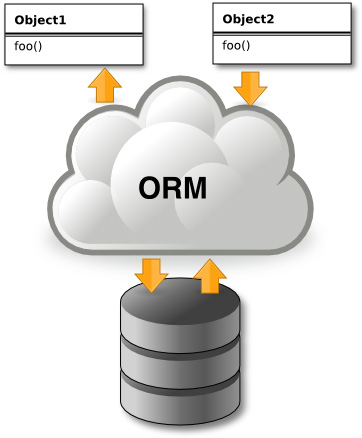
\includegraphics[scale=0.1]{img/ORM}
				\column{0.7\textwidth}
				\textbf{promotor:} dr inż. Arkadiusz Tomczyk
			\end{columns}
		\end{center}
	}
	\section{Problematyka pracy inżynierskiej}
  	\frame{
		\transboxin
   		\frametitle{Problematyka pracy inżynierskiej}
   		\framesubtitle{Czego praca ma dotyczyć, część praktyczna oraz teoretyczna}

   		\textbf{Praca inżynierska dotyczyć będzie:}
   		\begin{itemize}
   			\item<1-> zagadnień mapowania obiektowo-relacyjnego,
   			\item<2-> przystosowania programu C++ do wspierania mechanizmów retrospekcji,
   			\item<3-> zbudowanie niezależnej biblioteki jako bazy dla mechanizmu retrospekcji,
			\item<4-> rozpoznanie i wsparcie mechanizmów \textbf{implicit sharing} oraz \textbf{explicit sharing},
			\item<5-> obsługi błędów związanych z wykorzystaniem mechanizmów retrospekcji,   		
			\item<6-> zbudowania biblioteki współdzielonej wspierającej rozwiązanie końcowe   		
   		\end{itemize}
  	}
  	
  	\section{Istniejące rozwiązania wspierające refleksję}
  	\begin{frame}[fragile]
		\transboxin
    	\frametitle{Wykorzystanie refleksji w praktyce}
    	\framesubtitle{Kody źródłowe oraz opis}
    	\begin{columns}[c]
    		\column{.6\textwidth}
	    	\begin{block}{
\includegraphics[scale=0.1]{img/java}}
				\inputminted[
					linenos=true,
					fontsize=\tiny,
		            numbersep=2pt
				]{java}{listings/java_reflection}
	    	\end{block}\pause
	    	\begin{block}{
\includegraphics[scale=0.1]{img/python}}
				\inputminted[
					linenos=true,
					fontsize=\tiny,
		            numbersep=2pt
				]{python}{listings/python_reflection}	
	    	\end{block}\pause
	    	\begin{block}{
\includegraphics[scale=0.1]{img/logo_js}}
				\inputminted[
					linenos=true,
					fontsize=\tiny,
		            numbersep=2pt
				]{javascript}{listings/js_reflection}	
	    	\end{block}\pause
    		\column{.4\textwidth}
    		Cechą wspólną wszystkich tych rozwiązań jest
    		operowanie na instancja obiektów bez właściwej 
    		znajomości ich typu innej niż wiedza o nazwie
    		klasy bądź istnieniu konkretnej metody.
    	\end{columns}
	\end{frame}
  	
  	\section{Możliwe zastosowania refleksji}
  	\frame{
		\transboxin
    	\frametitle{Zastosowania refleksji}
    	\framesubtitle{O możliwych zastosowaniach}
    	\begin{enumerate}
    		\item \textbf{Paradygmat} - Programowanie zorientowane na refleksje \cite{ROP},
    		\item<2-> \textbf{Modyfikacja danych} - modyfikowanie obiektów bez właściwej znajomości ich typu,
    		jedynie na podstawie struktury wewnętrznej,
    		\item<3-> \textbf{Modyfikacja struktury} - dodawanie, usuwanie metod, zmiennych itp w czasie
    		wykonywania programu
    	\end{enumerate}
  	}
  	
  	\section{Plan pracy}
  	\frame{
		\transboxin
    	\frametitle{Plan pracy}
    	\framesubtitle{O zadaniach do wykonania}
    	\begin{block}{Problem}
    		\large{Uzyskanie efektywnego mechanizmu refleksji w C++}
    	\end{block}
    	\begin{block}{Rozwiązanie}
	    	\begin{enumerate}
	    		\item Poznanie mechanizmu meta obiektów w bibliotece Qt,
	    		\item<1-> Zrozumienie zasady działania \textbf{implicit} oraz \textbf{explicit} sharing
	    		\item<1-> Poznanie nowego standardu języka C++
	    		\item<2-> Zaprojektowanie niezależnej struktury klas jako meta modeli dla właściwej aplikacji
	    		\item<2-> Przystosowanie rozwiązania do wspierania mapowania obiektowo-relacyjnego.
	    	\end{enumerate}
    	\end{block}
  	}
  	
  	\section{Technologie, wzorce, architektura}
  	\frame{
		\transboxin
    	\frametitle{Technologie, wzorce, architektura}
    	\framesubtitle{O używanych technologiach, bibliotekach itp.}
    	\begin{block}{
\includegraphics[scale=0.06]{img/qt-logo}}
    		Skorzystanie z szeregu gotowych metod oraz obiektów,
    		wspierających meta programowanie, EDP\footnote{Event-Driven-Programming} oraz 
    		podstawowe mechanizmy refleksji pozwalający na modyfikowanie obiektów
    	\end{block}
    	\begin{columns}
    		\column{.5\textwidth}
	    	\begin{block}{Wzorce projektowe}
	    		Użycie szeregu wzorców celem stworzenie aplikacji modularnej,
	    		skalowalnej i łatwiej w debugowaniu.
	    	\end{block}
	    	\column{.5\textwidth}
	    	\begin{block}{Architektura}
	    		Biblioteka współdzielona\footnote{\textbf{SharedObject} lub \textbf{DLL}}
	    	\end{block}
    	\end{columns}
  	}
  	\note{EDP - programowanie wspierające event oraz listenery}
  	
  	\section{Bibliografia}
  	\frame[allowframebreaks]{
		\transboxin
	 	\frametitle<presentation>{Weiterf¸hrende Literatur}    
	 	\begin{thebibliography}{10}    
	  		\beamertemplatearticlebibitems
		  		\bibitem[Reflection-Oriented Programming]{ROP}
		    		Jonathan M. Sobel Daniel P. Friedman
		    	\newblock \em{Computer Science Department, Indiana University}.
		    	\newblock \href{http://www.cs.indiana.edu/~jsobel/rop.html}{Reflection-Oriented Programming}
	  		\beamertemplatearticlebibitems
		  		\bibitem[Reflection at Wiki]{Wiki_Reflection}
		  			Wikipedia Community
		    	\newblock \em{Reflection in computer programming}
		    	\newblock \href{http://en.wikipedia.org/wiki/Reflection_(computer_programming)}{Wiki - Computer reflection}.
	  \end{thebibliography}
	}
	
	\section{Pytania ?}
  	\frame{
		\transboxin
    	\frametitle{Pytania ?}
    	\framesubtitle{Czas pytać....}
    	\begin{center}
    		\LARGE{Macie jakieś pytania?}
    		
\includegraphics[scale=0.5]{img/question-mark}
    	\end{center}
  	}
\end{document}